\documentclass[a4paper,oneside,11pt]{book}
\usepackage{NWUStyle}
\usepackage{titlesec} % For redefining chapter title format
\usepackage{listings}

% Redefine chapter and section spacing
\titlespacing{\chapter}{0pt}{-50pt}{5pt} % Adjust the spacing as needed
\titlespacing{\section}{0pt}{10pt}{5pt} % Adjust the spacing as needed

\titleformat{\chapter}[display]
{\normalfont\huge\bfseries}{}{0pt}{\Huge}

\begin{document}
\Title{Cryptography project manual}
\Initials{A.}
\FirstName{Ashton}
\Surname{du Plessis}
\StudentNumber{34202676}
\Supervisor{Prof. Lynette Drevin}
\MakeTitle 
\pagenumbering{roman} 
\tableofcontents
\pagestyle{plain}
\cleardoublepage 
\pagenumbering{arabic} 

\chapter[General Information]{General Information}
\begin{figure}[h]
    \centering
    \makebox[\textwidth][c]{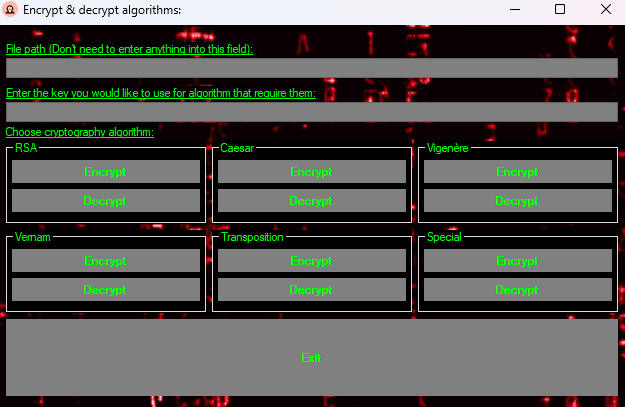
\includegraphics[width=1\textwidth, height=1\textheight, keepaspectratio]{Cryptography_Practical_Assignment_GUI.png}}
    \caption{GUI of Cryptography Application.}
\end{figure}

\chapter[RSA]{RSA}
\section{Encryption}
\begin{lstlisting}[language=Csh, caption={Code for RSA Encryption}]
public static bool EncryptFileRSA(string inputFile, string outputFile)
{
    try
    {
        GenerateRSAKeys(); // Generate RSA keys before encryption
        byte[] dataToEncrypt = File.ReadAllBytes(inputFile);
        List<byte[]> encryptedBlocks = new List<byte[]>();
    
        // Calculate the maximum block size for RSA encryption
        int blockSize = (publicKey.Modulus.Length / 8) - 11; 
    
        // Encrypt each block separately
        for (int i = 0; i < dataToEncrypt.Length; i += blockSize)
        {
            int remainingBytes = Math.Min(blockSize, 
            dataToEncrypt.Length - i);
            byte[] blockToEncrypt = new byte[remainingBytes];
            Array.Copy(dataToEncrypt, i, blockToEncrypt, 0, remainingBytes);    
            byte[] encryptedBlock = EncryptRSA(blockToEncrypt);
            encryptedBlocks.Add(encryptedBlock);
        }
    
        // Concatenate all encrypted blocks
        byte[] encryptedData = encryptedBlocks.SelectMany(x => x).ToArray();
        File.WriteAllBytes(outputFile, encryptedData);
        fileExtension = GetFileExtension(inputFile);
        return true; // Encryption completed successfully
    }
    catch (Exception ex)
    {
        // Log the exception or display an error message
        MessageBox.Show("Encryption failed: " + ex.Message);
        return false; // Encryption failed
    }
}
\end{lstlisting}

\subsection{Description of RSA Encryption}

The encryption algorithm for RSA works as follows:
The GenerateRSAKeys() method is called to generate public and private keys. By using File.ReadAllBytes() the contents of the input file is read into a byte array called dataToEncrypt. In order to calculate the maximum block size for this algorithm the length of the public key modulus is divided by 8 and then subtracted by 11. The file content is divided into blocks, these blocks is based on the block size that was calculated earlier. Each of the blocks is encrypted separately by the use of the EncryptRSA() method. Once a block has been encrypted it is stored in a list named encryptedBlocks. Once all of the blocks have been encrypted it is concatenated into a new single byte array called encryptedData by using LINQ's SelectMany() method. The File.WriteAllBytes() method is used to write the now concatenated data to an output file. If the encryption process is completed this method will return true to indicate that the encryption was successful. If any exception occurs during this process a message box will show on the screen stating that the encryption failed, and a false will be return to indicate that the encryption failed.

\section{Decryption}
\begin{lstlisting}[language=Csh, caption={Code for RSA Decryption}]
public static bool DecryptFileRSA(string inputFile, string outputFile)
{
    try
    {
        byte[] dataToDecrypt = File.ReadAllBytes(inputFile);
        byte[] decryptedData = DecryptRSA(dataToDecrypt, privateKey);
        File.WriteAllBytes(outputFile, decryptedData);
        return true;
    }
    catch(Exception ex)
    {
        MessageBox.Show("Decryption failed: " + ex.Message);
        return false;      
    }
}
\end{lstlisting}

\pagestyle{plain}
\subsection{Description of RSA Decryption}

The decryption algorithm for RSA works as follows:
By using File.ReadAllBytes() the completed of the input file is read into a byte array called dataToDecrypt. The encrypted data is decrypted by using the DecryptRSA() method by passing the dataToDecrypt array and the privateKey. The decrypted data is written to the output file by using the File.WriteAllBytes() method. If the decryption process is completed this method will return true to indicate that the decryption was successful. If any exception occurs during this process a message box will show on the screen stating that the decryption failed, and a false will be return to indicate that the decryption failed.

\chapter[Caeser Cipher]{Caeser Cipher}
\section{Encryption and Decryption}
\begin{lstlisting}[language=Csh, caption={Code for Encryption and Decryption of Caeser Cipher}]
private static byte CaesarCipher(byte inputByte, int key, bool encrypt)
{
    if (encrypt)
    {
        // Encryption: Shift the byte value by the key
        return (byte)((inputByte + key) % 256);
    }
    else
    {
        // Decryption: Shift the byte value backwards by the key
        return (byte)((inputByte - key + 256) % 256);
    }
}
    
// Function to encrypt or decrypt a binary file using the Caesar cipher
public static bool EncryptDecryptBinaryFile(string inputFile, 
string outputFile, int key, bool encrypt)
{
    try
    {
        // Open the input binary file for reading
        using (FileStream inputStream = new FileStream(inputFile, 
        FileMode.Open))
        {
            // Create a new binary writer to write to the output file
            using (BinaryWriter outputFileWriter = new BinaryWriter
            (File.Open(outputFile, FileMode.Create)))
            {
                // Read and process each byte in the input file
                int byteRead;
                while ((byteRead = inputStream.ReadByte()) != -1)
                {
                    // Encrypt or decrypt the byte using the Caesar cipher
                    byte processedByte = CaesarCipher((byte)byteRead, 
                    key, encrypt);
    
                    // Write the processed byte to the output file
                    outputFileWriter.Write(processedByte);
                }
            }
        }
        if (GetFileExtension(inputFile) != ".bin")
        {
            fileExtension = GetFileExtension(inputFile);
        }
        return true;
    }
    catch (Exception ex)
    {
        // If any exception occurs, return false
        Console.WriteLine($"An error occurred: {ex.Message}");
        return false;
    }
}
\end{lstlisting}

\subsection{Description of Caeser Cipher Encryption and Decryption}

The CaesarCipher() method determines if the input bytes are to be encrypted or decrypted. If it is to be encrypted the inputByte is added to the key and the result is then taken modulo 256 to ensure that it wraps around correctly within the byte range. The result of this calculation is caste to a byte and is return to be used in the main function for encrypting the input file. If it is not to be encrypted the key is subtracted from the inputByte, by adding 256 before taking the modulo 256 operation ensure that the result is always non-negative. The modulo operation ensures that the result wraps correctly around within the byte range. The result of this calculation is caste to a byte and is return to be used in the main function for decrypting the input file.

The main algorithm for this Caeser Cipher works as follows:
The input file is opened in read mode to read the concatenated of this file. The output is either created or overwritten and the file is being prepared to write binary data. A while loop is used to read each byte that is in the input file and the following is performed until the end of the file has bean reached:
\begin{itemize}
    \item 
        Each of the bytes that is read is processed by the CaesarCipher() method and to encrypt and to decrypt is determined by the encrypt flag that the EncryptDecryptBinaryFile() method receives. 
    \item 
        The bytes that have been processed is written into the output file.
\end{itemize}
If the encryption or decryption process is completed this method will return true to indicate that the encryption or decryption was successful. If any exception occurs during this process a message box will show on the screen stating that the encryption or decryption failed, and a false will be return to indicate that the encryption or decryption failed.

\chapter[Vigenère Cipher]{Vigenère Cipher}
\section{Encryption}
\begin{lstlisting}[language=Csh, caption={Code for Vigenère Cipher Encryption}]
public static bool VigenereEncryptBinaryFile(string inputFile, 
string outputFile, string key)
{
    try
    {
        byte[] dataToEncrypt = File.ReadAllBytes(inputFile);
        byte[] encryptedData = new byte[dataToEncrypt.Length];

        for (int i = 0; i < dataToEncrypt.Length; i++)
        {
            // Apply the Vigenere cipher algorithm
            int shift = key[i % key.Length] - 'A'; 
            encryptedData[i] = (byte)((dataToEncrypt[i] + shift) 
            % 256);
        }

        File.WriteAllBytes(outputFile, encryptedData);
        fileExtension = GetFileExtension(inputFile);
        return true;
    }
    catch (Exception ex)
    {
        Console.WriteLine("Encryption failed: " + ex.Message);
        return false;
    }
}
\end{lstlisting}

\subsection{Description of Vigenère Cipher Encryption}

The encryption algorithm for this Vigenère Cipher works as follows:
By using File.ReadAllBytes() the completed of the input file is read into a byte array called dataToEncrypt. A new byte array called encryptedData is created that will hold the encrypted bytes, this array has the same length as dataToEncrypt. By using a for loop to iterate through each byte in the dataToEncrypt array the following is applied to each byte:
\begin{itemize}
    \item 
        It calculates the shift based on the corresponding character in the key. The shift value is obtained by subtracting 'A' from the ASCII value of the character in the key. This assumes that the key contains uppercase alphabetic characters only.
    \item 
        It encrypts the byte by adding the shift value to the byte's value and taking the result modulo 256 (to ensure it stays within the byte range).
    \item 
        The encrypted byte is stored in the encryptedData array.
\end{itemize}
Once all of the bytes are encrypted the contents of the encryptedData array is written to the output file by using the File.WriteAllBytes() method. The global variable fileExtension is set to the file exception of the input file, to get the file exception of the input file the method GetFileExtension() is used. If the encryption process is completed this method will return true to indicate that the encryption was successful. If any exception occurs during this process a message box will show on the screen stating that the encryption failed, and a false will be return to indicate that the encryption failed.

\section{Decryption}

\begin{lstlisting}[language=Csh, caption={Code for Vigenère Cipher Decryption}]
public static bool VigenereDecryptBinaryFile(string inputFile, 
string outputFile, string key)
{
    try
    {
        byte[] dataToDecrypt = File.ReadAllBytes(inputFile);
        byte[] decryptedData = new byte[dataToDecrypt.Length];

        for (int i = 0; i < dataToDecrypt.Length; i++)
        {
            // Apply the Vigenere cipher algorithm
            int shift = key[i % key.Length] - 'A';
            decryptedData[i] = (byte)((dataToDecrypt[i] - shift + 256)
            % 256);
        }

        File.WriteAllBytes(outputFile, decryptedData);
        return true;
    }
    catch (Exception ex)
    {
        Console.WriteLine("Decryption failed: " + ex.Message);
        return false;
    }
}
\end{lstlisting}

\subsection{Description of Vigenère Cipher Decryption}

The decryption algorithm for this Vigenère Cipher works as follows:
By using File.ReadAllBytes() the completed of the input file is read into a byte array called dataToDecrypt. A new byte array called decryptedData is created that will hold the encrypted bytes, this array has the same length as dataToDecrypt. By using a for loop to iterate through each byte in the dataToDecrypt array the following is applied to each byte:
\begin{itemize}
    \item 
        It calculates the shift based on the corresponding character in the key. The shift value is obtained by subtracting 'A' from the ASCII value of the character in the key.
    \item 
        It decrypts the byte by subtracting the shift value from the byte's value, adding 256 to handle negative results, and then taking the result modulo 256 (to ensure it stays within the byte range).
    \item 
        The decrypted byte is stored in the decryptedData array.
\end{itemize}
Once all of the bytes are decrypted the contents of the decryptedData array is written to the output file by using the File.WriteAllBytes() method. If the decryption process is completed this method will return true to indicate that the decryption was successful. If any exception occurs during this process a message box will show on the screen stating that the decryption failed, and a false will be return to indicate that the decryption failed.

\chapter[Vernam Cipher]{Vernam Cipher}
\section{Encryption}
\begin{lstlisting}[language=Csh, caption={Code for Vernam Cipher Encryption}]
public static bool VernamEncryptBinaryFile(string inputFile, 
string outputFile, string key)
{
    try
    {
        // Read all bytes from the input file
        byte[] dataToEncrypt = File.ReadAllBytes(inputFile);
        byte[] encryptedData = new byte[dataToEncrypt.Length];
    
        // Perform Vernam encryption
        for (int i = 0; i < dataToEncrypt.Length; i++)
        {
            // Apply the Vernam cipher algorithm
            encryptedData[i] = (byte)(dataToEncrypt[i] ^ key
            [i % key.Length]);
        }
    
         // Write the encrypted data to the output file
        File.WriteAllBytes(outputFile, encryptedData);
        fileExtension = GetFileExtension(inputFile);
        return true;
    }
    catch (Exception ex)
    {
        MessageBox.Show("Encryption failed: " + ex.Message);
        return false;
    }
}
\end{lstlisting}

\subsection{Encryption of Vernam Cipher Encryption}

The encryption algorithm for this Vernam Cipher works as follows:
By using File.ReadAllBytes() the completed of the input file is read into a byte array called dataToEncrypt. A new byte array called encryptedData is created that will hold the encrypted bytes, this array has the same length as dataToEncrypt. By using a for loop to iterate through each byte in the dataToEncrypt array, a bitwise XOR (\^{}) operation is performed between each byte of the input data and the corresponding byte of the key. If the key is shorter than the input data it repeated, by using the modulus operator \% with the length of the key. The result of the XOR operation on the  dataToEncrypt array is stored in the encryptedData array. Once all of the bytes are encrypted the contents of the encryptedData array is written to the output file by using the File.WriteAllBytes() method. The global variable fileExtension is set to the file exception of the input file, to get the file exception of the input file the method GetFileExtension() is used. If the encryption process is completed this method will return true to indicate that the encryption was successful. If any exception occurs during this process a message box will show on the screen stating that the encryption failed, and a false will be return to indicate that the encryption failed.

\section{Decryption}
\begin{lstlisting}[language=Csh, caption={Code for Vernam Cipher Decryption}]
public static bool VernamDecryptBinaryFile(string inputFile, 
string outputFile, string key)
{
    try
    {
        // Read all bytes from the input file
        byte[] dataToDecrypt = File.ReadAllBytes(inputFile);
        byte[] decryptedData = new byte[dataToDecrypt.Length];
    
        // Perform Vernam decryption
        //(same as encryption because it's symmetric)
        for (int i = 0; i < dataToDecrypt.Length; i++)
        {
            // Apply the Vernam cipher algorithm
            decryptedData[i] = (byte)(dataToDecrypt[i] ^ 
            key[i % key.Length]);
        }
    
        // Write the decrypted data to the output file
        File.WriteAllBytes(outputFile, decryptedData);
        return true;
    }
    catch (Exception ex)
    {
        MessageBox.Show("Decryption failed: " + ex.Message);
        return false;
    }
}
\end{lstlisting}

\subsection{Description of Vernam Cipher Decryption}

The decryption algorithm of this Vernam Cipher works as follows:
By using File.ReadAllBytes() the completed of the input file is read into a byte array called dataToDecrypt. A new byte array called decryptedData is created that will hold the encrypted bytes, this array has the same length as dataToDecrypt. By using a for loop to iterate through each byte in the dataToDecrypt array, just like the encryption, a bitwise XOR (\^{}) operation is performed between each byte of the input data and the corresponding byte of the key. If the key is shorter than the input data it repeated, by using the modulus operator \% with the length of the key. The result of the XOR operation on the  dataToDecrypt array is stored in the decryptedData array. Once all of the bytes are encrypted the contents of the decryptedData array is written to the output file by using the File.WriteAllBytes() method. The global variable fileExtension is set to the file exception of the input file, to get the file exception of the input file the method GetFileExtension() is used. If the decryption process is completed this method will return true to indicate that the decryption was successful. If any exception occurs during this process a message box will show on the screen stating that the decryption failed, and a false will be return to indicate that the decryption failed.

\chapter[Transposition Cipher]{Transposition Cipher}

\section{Code needed to perform Encryption and Decryption of the Transposition Cipher}
\begin{lstlisting}[language=Csh, caption={Code for Transposition Cipher}]
// Function to get the permutation order based on the key
private static int[] GetPermutationOrder(string key)
{
    int[] permutationOrder = new int[key.Length];
    for (int i = 0; i < key.Length; i++)
    {
        permutationOrder[i] = i;
    }

    Array.Sort(key.ToCharArray(), permutationOrder);
    return permutationOrder;
}
\end{lstlisting}

\subsection{Description of code needed to perform Encryption and Decryption of the Transposition Cipher}
An array named permutationOrder is created, this array will hold the indices of the key in the sorted order thus the length of this array is the same as the length of the key. A for loop is used to initialise each element of the permutationOrder array, the total index is depended on the length of the key that is used. In order to sort the permutationOrder array the Array.Sort() method is used to sort this array by converting the key sting to a chapter array. The Array.Sort() method sorts the character array and rearranges the permutationOrder array in parallel to maintain the relative order of the original indices according to the sorted characters. The permutationOrder array will now contain indices that reflect the order of characters in the sorted key. The permutationOrder array is returned, to be used for encryption and decryption, the array now contains the indices of the key string and is sorted in ascending order of their corresponding characters.

\section{Encryption}
\begin{lstlisting}[language=Csh, caption={Code for Transposition Cipher Encryption}]
// Function to encrypt bytes using transposition cipher
private static byte[] TranspositionEncrypt(byte[] inputBytes, string key)
{
    int[] permutationOrder = GetPermutationOrder(key);

    int keyLength = key.Length;
    int numRows = (int)Math.Ceiling((double)inputBytes.Length 
    / keyLength);

    byte[,] matrix = new byte[numRows, keyLength];

    // Populate the matrix with input bytes
    for (int i = 0; i < inputBytes.Length; i++)
    {
        matrix[i / keyLength, i % keyLength] = inputBytes[i];
    }

    List<byte> encryptedBytes = new List<byte>();

    // Read the matrix column-wise according to permutation order
    foreach (int column in permutationOrder)
    {
        for (int row = 0; row < numRows; row++)
        {
            encryptedBytes.Add(matrix[row, column]);
        }
    }

    return encryptedBytes.ToArray();
}

// Function to encrypt a file using transposition cipher
public static bool TranspositionEncryptBinaryFile(string inputFile, 
string outputFile, string key)
{
    try
    {
        fileExtension = Path.GetExtension(inputFile);
        byte[] fileBytes = File.ReadAllBytes(inputFile);
        byte[] encryptedBytes = TranspositionEncrypt(fileBytes, key);
        File.WriteAllBytes(outputFile, encryptedBytes);
        return true;
    }
    catch (Exception ex)
    {
        Console.WriteLine("Error encrypting file: " + ex.Message);
        return false;
    }
}
\end{lstlisting}

\subsection{Description of Transposition Cipher Encryption}

The TranspositionEncrypt() method works as follows:
A array named permutationOrder is created and calls the GetPermutationOrder () method to obtain the permutation order that is based on the key. The number of rows needed to accommodate the input bytes when distributed into a matrix with columns equal to the length of the key is calculated. In order to keep the amount of rows needed an integer the Math.Ceiling() method is used. An array named matrix, with the number of rows equal to the numRows variable and the number of columns equal to the length of the key, is created. In order to populate the array, row-wise, with the input bytes a for loop is used, where i / keyLength determines the current row and i \% keyLength determines the current column. To store the encrypted bytes an empty list name encryptedBytes is initialised. Two for loops are used to iterate through each row, the inner for loop, in each column, the outer loop, and adding them to the encryptedBytes list. The encryptedBytes list is returned as an array to be used in the TranspositionEncryptBinaryFile() method.

The TranspositionEncryptBinaryFile() method works as follows:
The global variable fileExtension is set to the file exception of the input file, to get the file exception of the input file the method GetFileExtension() is used. A new byte array named fileBytes are created and the bytes from the input file is read into the array. A byte array named encryptedBytes is assigned the value that is returned by the TranspositionEncrypt() method, and takes the fileBytes array and the key as arguments. The content of the encryptedBytes array is written in to the output file. If the encryption process is completed this method will return true to indicate that the encryption was successful. If any exception occurs during this process a message box will show on the screen stating that the encryption failed, and a false will be return to indicate that the encryption failed.

\section{Decryption}
\begin{lstlisting}[language=Csh, caption={Code for Transposition Cipher Decryption}]
// Function to decrypt bytes using transposition cipher
private static byte[] TranspositionDecrypt(byte[] encryptedBytes, 
string key)
{
    int[] permutationOrder = GetPermutationOrder(key);

    int keyLength = key.Length;
    int numRows = (int)Math.Ceiling((double)encryptedBytes.Length 
    / keyLength);

    byte[,] matrix = new byte[numRows, keyLength];

    // Populate the matrix column-wise according to permutation order
    int encryptedIndex = 0;
    foreach (int column in permutationOrder)
    {
        for (int row = 0; row < numRows; row++)
        {
            matrix[row, column] = encryptedBytes[encryptedIndex++];
        }
    }

    List<byte> decryptedBytes = new List<byte>();

    // Read the matrix row-wise to obtain decrypted bytes
    for (int i = 0; i < numRows; i++)
    {
        for (int j = 0; j < keyLength; j++)
        {
            decryptedBytes.Add(matrix[i, j]);
        }
    }

    return decryptedBytes.ToArray();
}

// Function to decrypt a file using transposition cipher
public static bool TranspositionDecryptBinaryFile(string encryptedFile, 
string decryptedFile, string key)
{
    try
    {
        byte[] encryptedBytes = File.ReadAllBytes(encryptedFile);
        byte[] decryptedBytes = TranspositionDecrypt(encryptedBytes, key);
        File.WriteAllBytes(decryptedFile, decryptedBytes);
        return true;
    }
    catch (Exception ex)
    {
        Console.WriteLine("Error decrypting file: " + ex.Message);
        return false;
    }
}
\end{lstlisting}

\subsection{Description of Transposition Cipher Decryption}

The TranspositionDecrypt() method works as follows:
A array named permutationOrder is created and calls the GetPermutationOrder () method to obtain the permutation order that is based on the key. The number of rows needed to accommodate the encrypt bytes when distributed into a matrix with columns equal to the length of the key is calculated. In order to keep the amount of rows needed an integer the Math.Ceiling() method is used. An array named matrix, with the number of rows equal to the numRows variable and the number of columns equal to the length of the key, is created. In order to populate the matrix array column-wise according to the permutation order the encryptedIndex is first set to 0, and two for loops are used the outer for loop is used to populate the columns and the inner for loop is used to populate the rows of each of the columns. The encryptedIndex is iterated to move to the next byte. To store the decrypted bytes an empty list name decryptedBytes is initialised. Two for loops are used to iterate through each row, the inner for loop, in each column, the outer loop, and adding them to the decryptedBytes list. The decryptedBytes list is returned as an array to be used in the TranspositionDecryptBinaryFile() method.

The TranspositionDecryptBinaryFile() method works as follows:
A new byte array named encryptedBytes are created and the bytes from the encrypted file is read into the array. A byte array named decryptedBytes is assigned the value that is returned by the TranspositionDecrypt() method, and takes the encryptedBytes array and the key as arguments. The content of the decryptedBytes array is written in to the decrypted file. If the encryption process is completed this method will return true to indicate that the encryption was successful. If any exception occurs during this process a message box will show on the screen stating that the encryption failed, and a false will be return to indicate that the encryption failed.

\chapter[Special Cipher]{Special Cipher}

\section{Code needed to perform Encryption and Decryption of the Special Cipher}
\begin{lstlisting}[language=Csh, caption={Code for Special Cipher}]
private static RSAParameters publicKey;
private static RSAParameters privateKey;

public static void GenerateRSAKeys()
{
    using (var rsa = new RSACryptoServiceProvider(2048))
    {
        publicKey = rsa.ExportParameters(false);
        privateKey = rsa.ExportParameters(true); 
    }
}

public static byte[] GenerateAESKey()
{
    using (var aes = Aes.Create())
    {
        aes.GenerateKey();
        return aes.Key;
    }
}
\end{lstlisting}

\subsection{Description of code needed to perform Encryption and Decryption of the Special Cipher}

RSAParameters is a structure that holds the parameters for the RSA algorithm, including the modulus and exponent for the public key and additional parameters for the private key. The RSA public and private keys are stored in the publicKey and privateKey respectively. The GenerateRSAKeys() method generates a new RSA key pair. A new instance of the RSACryptoServiceProvider class is created with key size of 2048 bits. The public key parameters are exported, with the false that indicate that only the public key must be exported. Both the public and private keys are exported, with the true that indicate that the private part of the key must also be included. The GenerateAESKey() method generates a new AES key. A new instance of the default implementation of the AES algorithm is generated. aes.GenerateKey() is used to generate a random key that will be used in the AES algorithm, this key is returned, as a byte array, to be used latter.

\section{Encryption}
\begin{lstlisting}[language=Csh, caption={Code for Special Cipher Encryption}]
public static byte[] EncryptRSA(byte[] data)
{
    using (var rsa = new RSACryptoServiceProvider())
    {
        rsa.ImportParameters(publicKey);
        return rsa.Encrypt(data, RSAEncryptionPadding.Pkcs1);
    }
}

public static byte[] EncryptAES(byte[] data, byte[] key)
{
    using (var aes = Aes.Create())
    {
        aes.Key = key;
        using (var encryptor = aes.CreateEncryptor())
        {
            using (MemoryStream ms = new MemoryStream())
            {
                using (CryptoStream cs = new CryptoStream(ms, 
                encryptor, CryptoStreamMode.Write))
                {
                    cs.Write(data, 0, data.Length);
                    cs.FlushFinalBlock();
                }
                return ms.ToArray();
            }
        }
    }
}

public static bool EncryptFileHybrid(string inputFile, 
string outputFile)
{
    try
    {
        GenerateRSAKeys(); // Generate RSA keys before encryption
        byte[] aesKey = GenerateAESKey();
        byte[] encryptedAESKey = EncryptRSA(aesKey);
    
        byte[] dataToEncrypt = File.ReadAllBytes(inputFile);
    
        using (Aes aesAlg = Aes.Create())
        {
            aesAlg.Key = aesKey;
            aesAlg.GenerateIV(); // Generate IV
            byte[] iv = aesAlg.IV;
    
            using (MemoryStream ms = new MemoryStream())
            {
                // Write IV to the beginning of the MemoryStream
                ms.Write(iv, 0, iv.Length);
    
                using (CryptoStream cs = new CryptoStream
                (ms, aesAlg.CreateEncryptor(), CryptoStreamMode.Write))
                {
                    // Write encrypted data to the CryptoStream
                    cs.Write(dataToEncrypt, 0, dataToEncrypt.Length);
                    cs.FlushFinalBlock();
                }
                byte[] encryptedData = ms.ToArray();
    
                using (var combinedStream = new MemoryStream())
                {
                    combinedStream.Write(encryptedAESKey, 0, 
                    encryptedAESKey.Length);
                    combinedStream.Write(encryptedData, 0, 
                    encryptedData.Length);
    
                    File.WriteAllBytes(outputFile, combinedStream.ToArray());
                }
            }
        }
        fileExtension = GetFileExtension(inputFile);
        return true; // Encryption completed successfully
    }
    catch (Exception ex)
    {
        // Log the exception or display an error message
        MessageBox.Show("Encryption failed: " + ex.Message);
        return false; // Encryption failed
    }
}
\end{lstlisting}

\subsection{Description of Special Cipher Encryption}

The EncryptRSA() method for this encryption method works as follows:
A new instance of the RSA cryptographic service provider is initialised. The The public RSA parameters that are stored in publicKey is imported. The encrypted input data is returned. This data in encrypted by using the RSA public key with PKCS\#1 padding.

The EncryptAES() method for this encryption method works as follows:
A new instance of AES algorithm is created. The encryption key for the AES instance is set. A symmetric encryptor object with the specified key and initialization vector is created, if a initialization vector is not specified it is created automatically. A memory stream that holds the encrypted data is created. A CryptoStream that links the memory stream to the AES encryptor is created, which will handle the encryption process. Input data is written to the CryptoStream, which encrypts it and writes the encrypted data to the memory stream. cs.FlushFinalBlock() ensures that all data is written and the encryption process is completed. This method is necessary to finalize the encryption process and ensure the integrity of the encrypted data. The memory stream is converted to a byte array, which contains the encrypted data. This byte array is than returned to be used latter.

The EncryptFileHybrid() method, which is the method that combines the above mentioned methods, works as follows:


\section{Decryption}
\begin{lstlisting}[language=Csh, caption={Code for Special Cipher Decryption}]
public static byte[] DecryptRSA(byte[] data, RSAParameters privateKey)
{
    using (var rsa = new RSACryptoServiceProvider())
    {
        rsa.ImportParameters(privateKey);
        return rsa.Decrypt(data, RSAEncryptionPadding.Pkcs1);
    }
}

public static byte[] DecryptAES(byte[] data, byte[] key)
{
    using (var aes = Aes.Create())
    {
        aes.Key = key;
        using (var decryptor = aes.CreateDecryptor())
        {
            using (MemoryStream ms = new MemoryStream())
            {
                using (CryptoStream cs = new CryptoStream(ms, decryptor, 
                CryptoStreamMode.Write))
                {
                    cs.Write(data, 0, data.Length);
                    cs.FlushFinalBlock();
                }
                return ms.ToArray();
            }
        }
    }
}

public static bool DecryptFileHybrid(string inputFile, string outputFile)
{
    try
    {
        byte[] encryptedData = File.ReadAllBytes(inputFile);
        byte[] encryptedAESKey = new byte[256];
        byte[] encryptedDataWithoutKey = new byte
        [encryptedData.Length - 256];
    
        Array.Copy(encryptedData, encryptedAESKey, 256);
        Array.Copy(encryptedData, 256, encryptedDataWithoutKey, 
        0, encryptedData.Length - 256);
    
        byte[] aesKey = DecryptRSA(encryptedAESKey, privateKey);
    
        using (Aes aesAlg = Aes.Create())
        {
            aesAlg.Key = aesKey;
    
            // Extract IV from the beginning of the encryptedData
            byte[] iv = new byte[aesAlg.IV.Length];
            Array.Copy(encryptedDataWithoutKey, iv, aesAlg.IV.Length);
            aesAlg.IV = iv;
    
            using (MemoryStream ms = new MemoryStream
            (encryptedDataWithoutKey, aesAlg.IV.Length, 
            encryptedDataWithoutKey.Length - aesAlg.IV.Length))
            {
                using (CryptoStream cs = new CryptoStream(ms, 
                aesAlg.CreateDecryptor(), CryptoStreamMode.Read))
                {
                    using (MemoryStream decryptedStream = new MemoryStream())
                    {
                        cs.CopyTo(decryptedStream);
                        File.WriteAllBytes(outputFile, 
                        decryptedStream.ToArray());
                    }
                }
            }
        }
        return true;
    }
    catch (Exception ex)
    {
        MessageBox.Show("Decryption failed: " + ex.Message);
        return false;
    }
}
\end{lstlisting}

\subsection{Description of Special Cipher Decryption}



\end{document}
